\documentclass[tikz, border=0pt]{standalone}
\usepackage{amsmath}
\usetikzlibrary{calc, intersections, arrows.meta}

\begin{document}
\sffamily
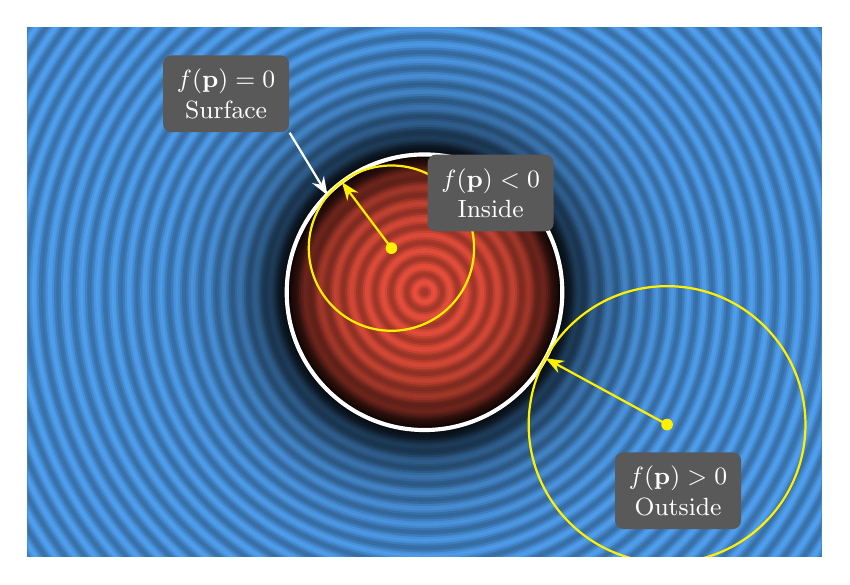
\begin{tikzpicture}[scale=1.4, >=Stealth]
  % Clip the scene to a nice rectangle with NO outer margin
  \clip (-3.6, -2.4) rectangle (3.6, 2.4);

  % ==========================================
  % 1. SHADER COLORS & SETUP
  % ==========================================
  % Base colors corresponding to the Shadertoy visual
  \definecolor{blueBase}{RGB}{80, 160, 240} % Bluish outside
  \definecolor{redBase}{RGB}{235, 80, 60}   % Reddish inside
  \definecolor{sdfYellow}{RGB}{255, 240, 0} % Probe rings

  \def\R{1.25} % Surface radius
  \coordinate (Center) at (0,0);
  
  % Invisible path for the surface used for exact intersections later
  \path[name path=surf] (Center) circle (\R);

  % ==========================================
  % 2. RENDER OUTSIDE (f(p) > 0)
  % ==========================================
  % Draw concentric circles converging towards the boundary
  \foreach \r in {5.00, 4.98, ..., 1.26} {
    \pgfmathsetmacro{\d}{\r - \R}
    
    % Mimic IQ's shader: 1.0 - exp(-k * abs(d))
    \pgfmathsetmacro{\darken}{1.0 - exp(-3.0 * \d)}
    % Mimic IQ's contour ripples: 0.8 + 0.2*cos(...)
    \pgfmathsetmacro{\wave}{0.85 + 0.15*cos(2500 * \d)}
    
    % Calculate final intensity (0 to 100)
    \pgfmathsetmacro{\intensity}{max(0, min(100, int(round(100 * \darken * \wave))))}
    
    \colorlet{mycol}{blueBase!\intensity!black}
    \fill[mycol] (Center) circle (\r);
  }

  % ==========================================
  % 3. RENDER INSIDE (f(p) < 0)
  % ==========================================
  \foreach \r in {1.24, 1.22, ..., 0.02} {
    \pgfmathsetmacro{\d}{\R - \r}
    
    \pgfmathsetmacro{\darken}{1.0 - exp(-4.0 * \d)}
    \pgfmathsetmacro{\wave}{0.85 + 0.15*cos(2500 * \d)}
    \pgfmathsetmacro{\intensity}{max(0, min(100, int(round(100 * \darken * \wave))))}
    
    \colorlet{mycol}{redBase!\intensity!black}
    \fill[mycol] (Center) circle (\r);
  }

  % ==========================================
  % 4. SURFACE ZERO-CROSSING (f(p) = 0)
  % ==========================================
  \draw[white, line width=1.5pt] (Center) circle (\R);

  % ==========================================
  % 5. SDF PROBES (Mimicking iMouse interaction)
  % ==========================================
  % --- Outside Probe ---
  \coordinate (Pout) at (2.2, -1.2);
  \path[name path=rayOut] (Center) -- (Pout);
  \path[name intersections={of=rayOut and surf, by=Sout}];
  
  % Draw the exact distance ring tangent to the surface
  \draw[sdfYellow, thick] (Pout) let \p1 = ($(Pout)-(Sout)$), \n1 = {veclen(\x1,\y1)} in circle (\n1);
  \draw[sdfYellow, thick, -Stealth] (Pout) -- (Sout);
  \fill[sdfYellow] (Pout) circle (1.5pt);

  % --- Inside Probe ---
  \coordinate (Pin) at (-0.3, 0.4);
  % Extend the line outward to find the nearest surface point from the inside
  \path[name path=rayIn] (Center) -- ($ (Center)!5!(Pin) $);
  \path[name intersections={of=rayIn and surf, by=Sin}];
  
  \draw[sdfYellow, thick] (Pin) let \p1 = ($(Sin)-(Pin)$), \n1 = {veclen(\x1,\y1)} in circle (\n1);
  \draw[sdfYellow, thick, -Stealth] (Pin) -- (Sin);
  \fill[sdfYellow] (Pin) circle (1.5pt);

  % ==========================================
  % 6. ANNOTATIONS
  % ==========================================
  \tikzset{
    labelbox/.style={
      fill=black!65, text=white, rounded corners=3pt, inner sep=5pt, 
      align=center, font=\small
    }
  }

  % Float labels dynamically next to the probes
  \node[labelbox] at (2.3, -1.8) {$f(\mathbf{p}) > 0$\\Outside};
  \node[labelbox] at (0.6, 0.9) {$f(\mathbf{p}) < 0$\\Inside};
  
  \node[labelbox] (surfNode) at (-1.8, 1.8) {$f(\mathbf{p}) = 0$\\Surface};
  \draw[white, thick, -Stealth] (surfNode.south east) -- (-0.88, 0.88);

  % Footer Description
  % \node[labelbox, fill=black!85, font=\footnotesize] at (0, -2.1)
  %   {An SDF returns the exact signed distance to the nearest boundary.\\The yellow rings show this safe stepping distance during raymarching.};

\end{tikzpicture}
\end{document}